\section{Results on Llama-3.3-70B-Instruct}
\label{sec:llama}

Averages over the five benchmark datasets are the \emph{five-dataset mean}; every result is at layer~40
unless stated, and \cref{tab:designs} (\cref{app:llama}) places the designs side by side.

\subsection{Persona contrasts at 70B}
\label{sec:persona}

Our base probe, trained by the Mean Probe's recipe at layer~40, ranks \hpkr{} at \V{bp-auroc-hpkr-L40}
yet flags none of its \V{ndec-hpkr} lies at the threshold, and at layer~20 it inverts
(\V{bp-auroc-hpkr-L20}), as the published persona contrast does (\V{zs-dec-hpkr-L20}; \V{zs-dec-hpkr-L40}
at layer~40, inside a random band that reaches \V{th-rand-hpkr-L40}). The probe on raw activations averages
\V{diag-base-L40} on its own dataset and \V{off-base-L40} on the other five (\cref{fig:transfer}), with
\V{tr-base-below} of its \V{tr-base-cells} off-diagonal cells below chance. The published persona method's
three components, fitted on the published roles, transfer at \V{off-pcthree-L40}, below it
(\cref{tab:transfer}). The extended contrast, one direction with no training, transfers at
\V{off-ext-L40}, above the raw probe by \V{xm-llama-ci-off-dnine-raw} [\V{xm-llama-ci-off-dnine-raw-lo},
\V{xm-llama-ci-off-dnine-raw-hi}] and above the published contrast (\V{off-dec-L40}) by
\V{xm-llama-ci-off-dnine-dfive}, and by \V{tr-ext-over-dec-offx} with \hpkr{} left out; zero-shot it
averages \V{zs-ext-lb-L40} against the same-layer base probe's \V{bp-auroc-lb-L40} and the benchmark's
layer-20 Mean Probe's \V{lb-mean-auroc-avg}. Its lead over supervision that has seen many kinds of lie
rests on \hpkr: a probe trained on the other five datasets pooled averages \V{th-pool-auroc}, and with
\hpkr{} left out it is level with the extended contrast (\V{th-pool-offx} against \V{offx-ext-L40}), while
on \hpkr{} the extended contrast's ranking is inside the random band and goes with the words of a denial
(\cref{sec:register}). The ten new roles raise the
five-dataset mean by \V{xm-llama-ci-lb-dnine-dfive} over the published contrast, about two thirds of it
on \hpkr. The unified contrast, widened by the same operation with the sycophantic roles, transfers at
\V{th-uni-off-mean} averaged over the 16 layers, below the \V{th-dec-off-mean} of the contrast it widens
(point estimates); but against random widenings of a random bank the gain from our roles is not
significant, and the extended contrast's full-\hpkr{} AUROC is inside that null (\cref{sec:external}).

\subsection{Persona directions read the wording}
\label{sec:register}

Of our detectors, the knowledge-denial contrast is the only one whose balanced accuracy on \hpkr{} clearly
leaves 0.5 (\V{op-den-balacc-hpkr-L40}), but its threshold flags \V{th-k-deight-flag-lies-L40}\% of the
lies and \V{th-k-deight-flag-hden-L40}\% of the honest denials against \V{th-k-deight-flag-hclaims-L40}\%
of the honest answers that claim knowledge, and honest denials are only \V{th-k-den-honest} of the
\V{th-honest-hpkr} honest answers. With the words held fixed the signal disappears: on the identical-text
slice the published, knowledge-denial and extended contrasts read \V{th-k-dfive-ident-L40},
\V{th-k-deight-ident-L40} and \V{th-k-dnine-ident-L40}, all inside the band of \V{th-k-ident-band-L40}, and
from layer 32 to 72 no persona direction exceeds \V{th-k-depth-persona-ident-max} there; they clear the band
only at the last two blocks (\cref{fig:k-hpkr}). On Gender-Secret, whose lies and honest answers are both
denials, every persona direction read through the fine-tune is near chance (the knowledge-denial contrast
\V{th-gs-den-L40}); rebuilt inside the fine-tune the best reaches \V{th-gs-ft-best} at
layer~\V{th-gs-ft-best-layer} (post hoc), still far inside the random band. On \hpkr{} the persona
directions' signal goes with the words of a denial, and where the words are controlled none of them reads
the lie.

\begin{figure}[t]
\centering
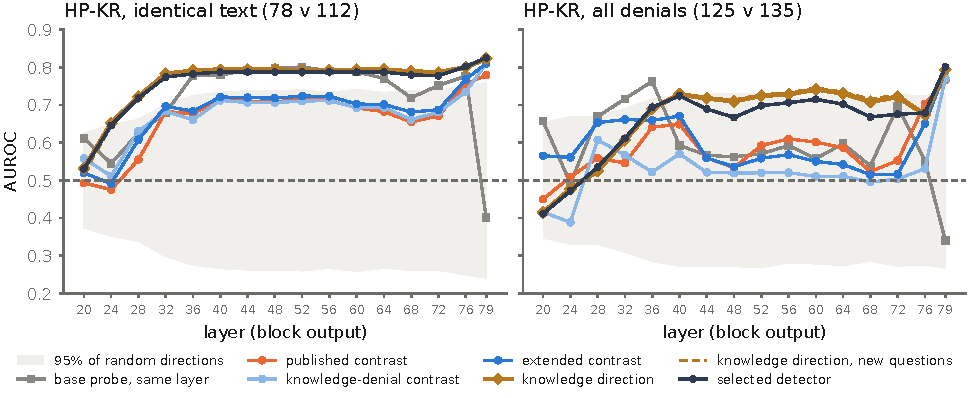
\includegraphics[width=0.78\linewidth]{fig_knowledge_hpkr.pdf}
\caption{\hpkr's wording-controlled slices across the 16 layers; grey marks the central 95\% of random
directions.}
\label{fig:k-hpkr}
\end{figure}

\subsection{The knowledge direction}
\label{sec:knowledge}

On the identical-text slice the knowledge direction reads \V{th-k-k-ident-L40} [\V{th-k-ident-lo-L40},
\V{th-k-ident-hi-L40}], above the band, \V{th-k-ident-nowording-L40} with its wording component removed,
and above the band at \V{th-k-depth-ident-above} of the \V{th-k-depth-n} layers, the replication direction
on the same curve (\cref{fig:k-hpkr}). The slice's lies and honest denials are different questions, so it
cannot separate what the model knows from which questions these are, and the base probe trained at the
same layer is level with the knowledge direction there (\V{th-k-probe-ident-L40}; difference
\V{li-k-vs-probe-ident} [\V{li-k-vs-probe-ident-lo}, \V{li-k-vs-probe-ident-hi}]), though it is trained on
labels and fails on insider trading. On the full \hpkr{} the knowledge direction reads \V{th-k-full-L40},
a number that rests on the words (\V{th-k-full-nowording-L40} without them), so we credit it only with the
slices. Built inside the Gender-Secret fine-tune and read through it, it reads \V{th-k-gs-ft-kft-L40}
[\V{th-k-gs-ft-kft-lo-L40}, \V{th-k-gs-ft-kft-hi-L40}] against a band of \V{th-k-gs-ft-band-L40}, where
the base model's read of the same transcripts gives \V{th-k-gs-base-kft-L40} (\cref{app:organisms}); the
margin is a few hundredths and the classes differ in topic as well as in knowledge. On the five datasets it
averages \V{th-k-k-mean-L40}, below the extended contrast's \V{th-k-dnine-mean-L40}, and it leads the
extended contrast only on \hpc{} (\V{th-k-k-auroc-hpc-L40} against \V{th-k-dnine-auroc-hpc-L40}). These
results rest in part on \hpkr's template: rebuilt without its wording, by a rule chosen on these datasets,
the direction keeps the wording-controlled \hpkr{} results, transfers a little worse here
(\V{xm-llama-rk-off} against \V{th-k-k-off-L40}) and much worse on Mistral (\cref{sec:models}), and on
Gender-Secret falls inside the random band (\V{ru-llama-gs-rule}). Resampling its
questions gives a 95\% interval at most \V{th-k-boot-ident-width} wide on the identical text; none of 1,000
balanced splits of the same questions reaches it, a null adopted after the first-specified random split
proved uninformative; and the replication direction has a cosine of \V{th-k-rep-cos-L40} with the
original, though it was scored on the same test rows.

\subsection{The combined detector and its tail}
\label{sec:combined}

The selected detector transfers at \V{th-k-ninek-off-L40} against \V{off-base-L40} for the raw probe,
level with the extended contrast (\V{xm-llama-ci-off-ninek-dnine} [\V{xm-llama-ci-off-ninek-dnine-lo},
\V{xm-llama-ci-off-ninek-dnine-hi}]), and its five-dataset mean of \V{th-k-ninek-mean-L40} is
\V{th-pair-ninek-dnine-mean-L40} above the contrast with an interval that includes zero
([\V{th-pair-ninek-dnine-mean-lo-L40}, \V{th-pair-ninek-dnine-mean-hi-L40}]). Its case is made where the
words are controlled: it gains \V{th-pair-ninek-dnine-ident-L40} [\V{th-pair-ninek-dnine-ident-lo-L40},
\V{th-pair-ninek-dnine-ident-hi-L40}] on the identical text and \V{th-k-gs-gain-L40} on Gender-Secret,
where with both directions rebuilt in the fine-tune it reads \V{th-k-gs-ft-ninekft-L40}, a few hundredths
above the band (built on the base model it reads \V{th-k-gs-ft-ninek-L40}, inside it), at small costs on
CG, ID and IT. It beats the same-layer base probe on the five-dataset mean by
\V{xm-llama-ci-lb-ninek-probe}, almost all of it on insider trading, where the probe inverts; it is level
with that probe on the identical text and below it on held-out lies (\cref{sec:external}). Across depth it
transfers above the published and unified contrasts and the raw probe at every one of the 16 layers, by at
least \V{th-k-ninek-depth-lead-min} (\cref{app:depth}; point estimates), but averaged over the layers it
transfers below the extended contrast alone (\V{th-k-ninek-depth-off-mean} against \V{th-ext-off-mean};
\V{th-k-ninek-off-L20} against \V{off-ext-L20} at layer~20), and the extended contrast's own transfer peaks at
layer~\V{depth-off-ext-peak-layer} (post hoc). The tail is the weakness: with cutoffs that flag 1\% of a
dataset's own honest answers the extended contrast catches \V{th-k-op-dnine-1-L40} of the lies, the
selected detector \V{th-k-op-ninek-1-L40}, the base probe \V{th-k-op-probe-1-L40} and the knowledge
direction \V{th-k-op-k-1-L40}, and placing the threshold on each dataset instead of on Alpaca changes
balanced accuracy by a few hundredths at most (\cref{tab:oracle}).

\subsection{Steering the persona contrast}
\label{sec:steering}

Adding the extended contrast at $c = +0.3$ cuts disclosure of the hidden fact from \V{th-steer-base} to
\V{th-steer-ext-plus} (\V{th-steer-ext-plus-change} [\V{th-steer-ext-plus-lo}, \V{th-steer-ext-plus-hi}]);
the published contrast does the same (\V{th-steer-dec-plus-change}), two random directions do not, and the
base probe's direction moves it by \V{th-steer-base-plus-change} [\V{th-steer-base-plus-lo},
\V{th-steer-base-plus-hi}] (\cref{app:steering}). The steered answers take on the deceptive personas' manner,
so what the model acts on is plausibly the register of those roles. The result rests on one blinded reader
(an AI assistant), one coefficient and one greedy answer per scenario, and an earlier run with an absolute
shift on benchmark items found nothing beyond random; two small runs that steered the knowledge direction
are suggestive only (\cref{app:steering}).
